\documentclass[11pt]{beamer}
\usetheme{bars}
\usepackage{xcolor}
\usepackage[utf8x]{inputenc}
\usepackage{ucs}
\usepackage[spanish]{babel}
\usepackage{amsmath}
\usepackage{amsfonts}
\usepackage{amssymb}
\usepackage{multicol}
\usepackage{graphicx}
\usepackage{multicol}
\graphicspath{{Figures/}}
%\setbeamercovered{transparent} 
\definecolor{colorZ}{RGB}{0,60,127}
\usecolortheme[RGB={0,60,127}]{structure}
\setbeamertemplate{navigation symbols}{}
\setbeamercolor{mycolor}{bg=colorZ,fg=white}
\defbeamertemplate*{footline}{shadow theme}{%
\leavevmode%
\hbox{\begin{beamercolorbox}[wd=.5\paperwidth,ht=2.5ex,dp=1.125ex,leftskip=.3cm plus1fil,rightskip=.3cm]{author in head/foot}%
    \usebeamerfont{author in head/foot}\hfill\insertshortauthor
\end{beamercolorbox}%
\begin{beamercolorbox}[wd=.43\paperwidth,ht=2.5ex,dp=1.125ex,leftskip=.3cm,rightskip=.3cm plus1fil]{title in head/foot}%
    \usebeamerfont{title in head/foot}\insertshorttitle\hfill%
\end{beamercolorbox}%
\begin{beamercolorbox}[wd=.07\paperwidth,ht=2.5ex,dp=1.125ex,leftskip=.1cm,rightskip=.1cm plus1fil]{mycolor}%
\hfill\insertframenumber\,/\,\inserttotalframenumber
\end{beamercolorbox}}%
\vskip0pt%
}
\author[Daniel Osorio]{\textbf{Daniel Osorio}\inst{1,2,3} \and \textbf{Janneth Gonzalez}\inst{2} \and \textbf{Andrés Pinzon}\inst{3}}
\title[Bioinformatics Master Thesis]{Identifying proteins and metabolic pathways associated with the neuroprotective response mediated by tibolone in astrocytes under an induced inflammatory model}
\institute[]{\inst{1} Departamento de Ingeniería de Sistemas e Industrial\\Facultad de Ingeniería, Universidad Nacional de Colombia \and \inst{2} Grupo de Investigación en Bioquímica Experimental y Computacional\\Facultad de Ciencias, Pontificia Universidad Javeriana - Bogotá \and \inst{3} Grupo de Investigación en Bioinformática y Biología de Sistemas\\ Instituto de Genética, Universidad Nacional de Colombia} 
\date[]{\scriptsize{\textbf{Universidad Nacional de Colombia, November 2016}}}
\begin{document}
\maketitle
\section{Introduction}
\begin{frame}

\end{frame}
\section{Objectives and Methods}
\begin{frame}

\end{frame}
\section{Results}
\begin{frame}{Age Related Metabolic Changes in Astrocytes}
\begin{center}
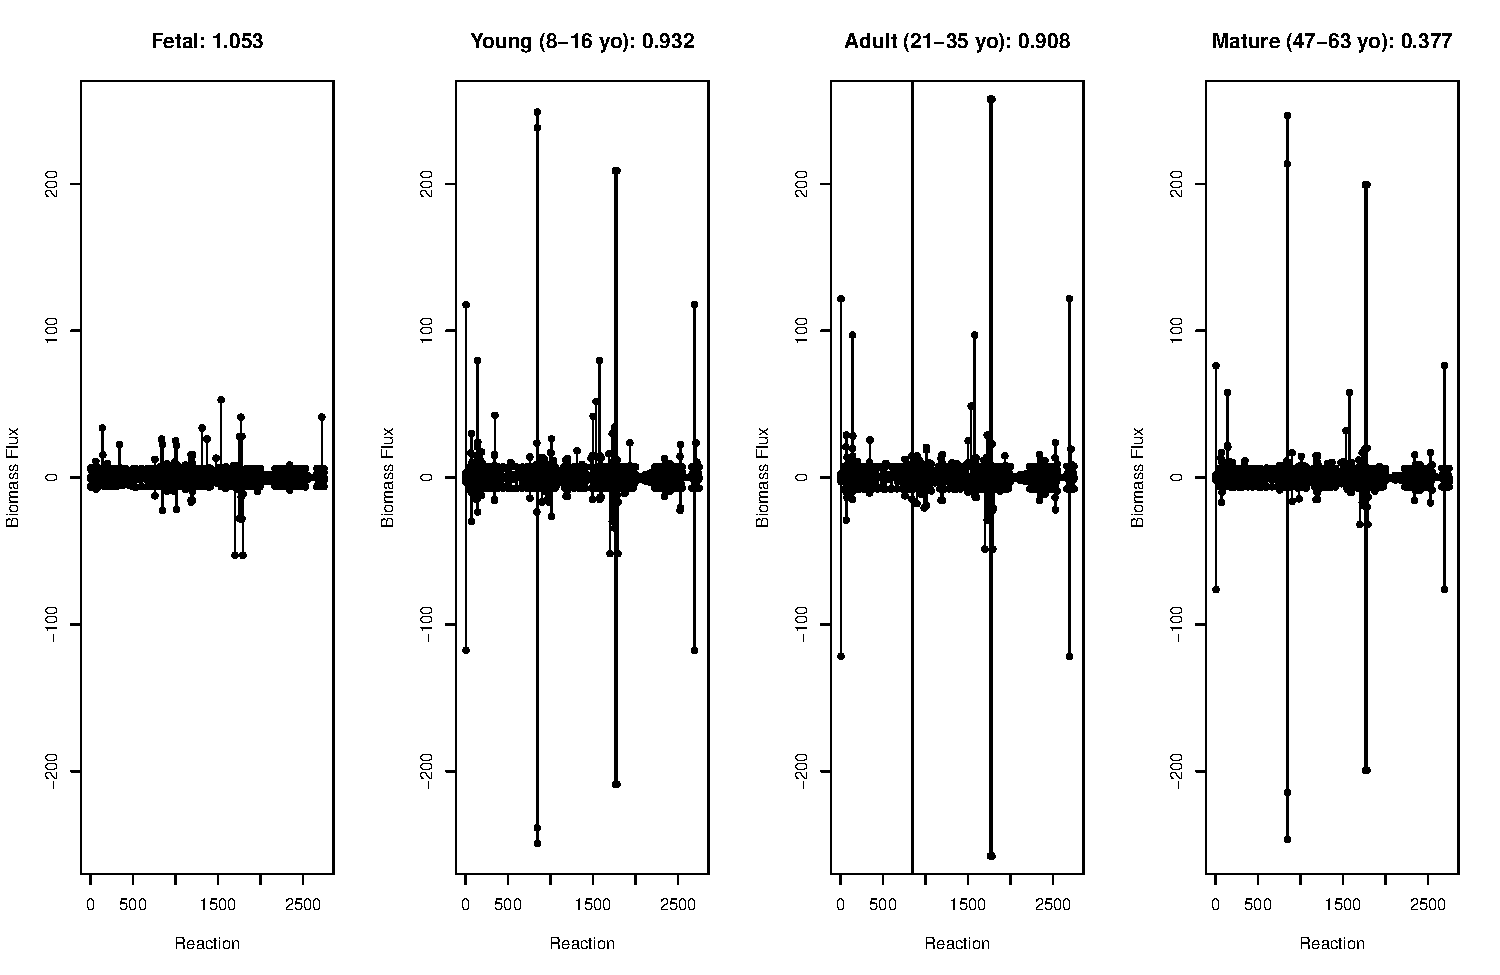
\includegraphics[width=\textwidth]{Astrocyte_MetabolicChanges}
\end{center}
\end{frame}
\begin{frame}{IC$_{50}$ = 0.214 $\pm$ 0.016 mMgDW$^{-1}$h$^{-1}$}
\begin{center}
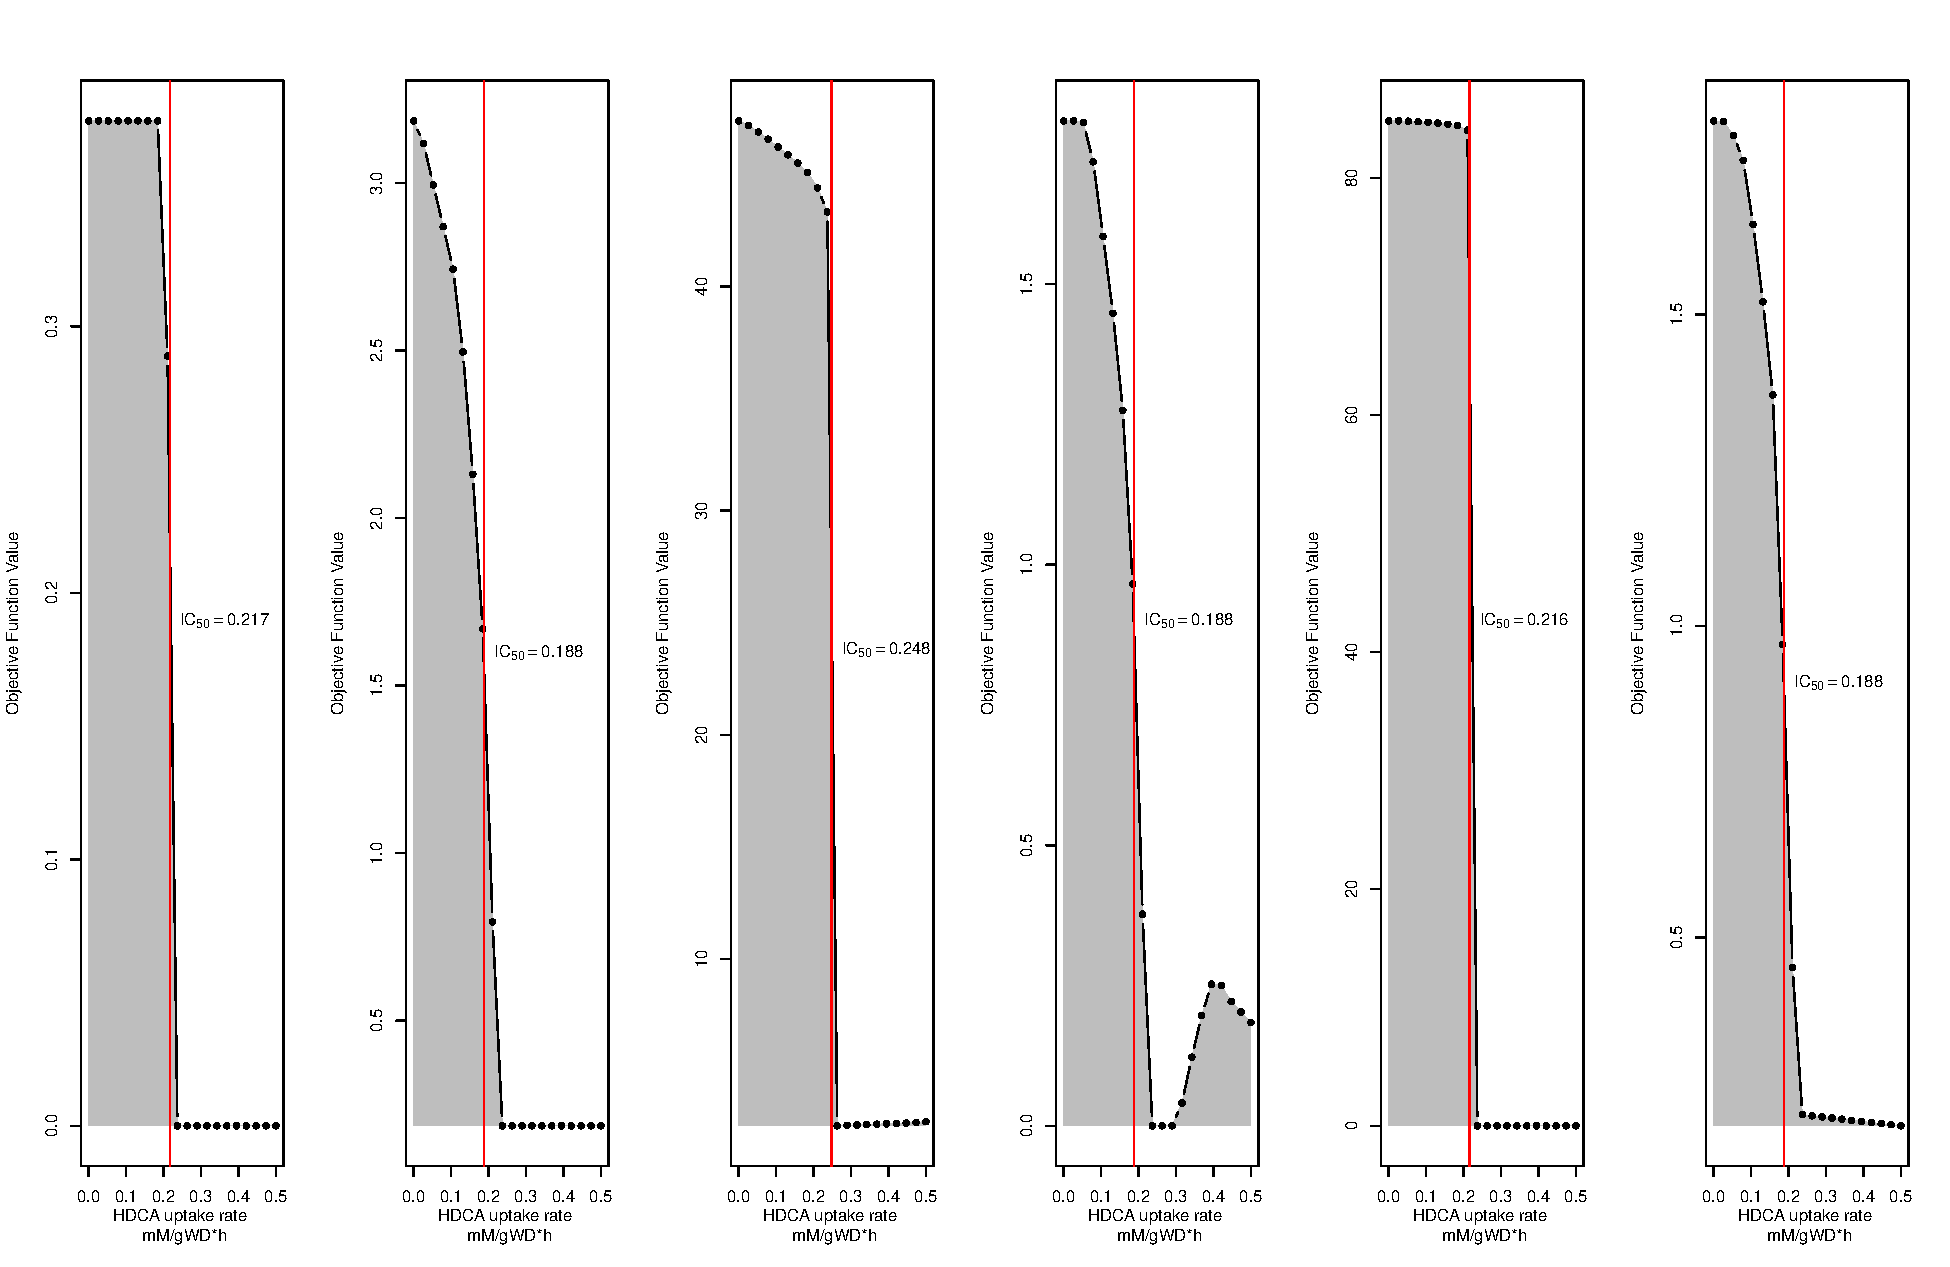
\includegraphics[width=\textwidth]{IC50}
\end{center}
\end{frame}
\begin{frame}{Software Development}
\begin{center}
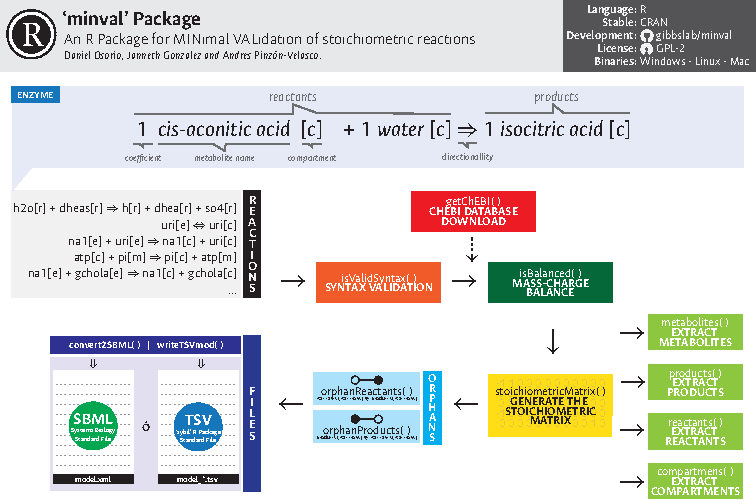
\includegraphics[width=\textwidth]{minval}
\end{center}
\end{frame}
\begin{frame}{Software Development}
\begin{center}
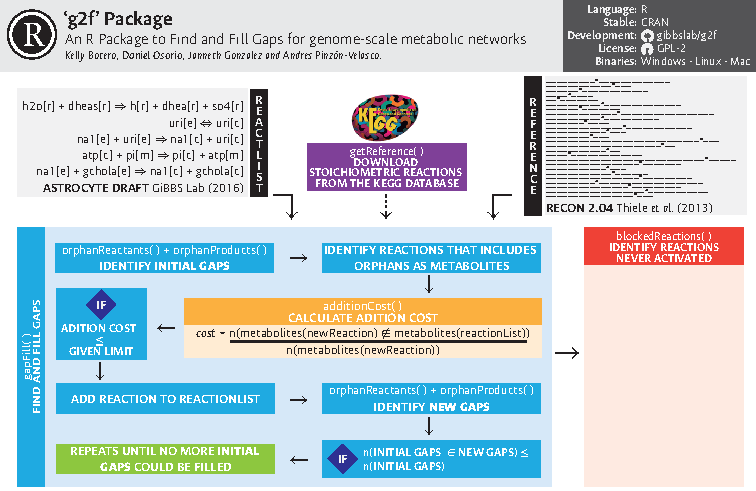
\includegraphics[width=\textwidth]{g2f}
\end{center}
\end{frame}
\begin{frame}{Software Development}
\begin{center}
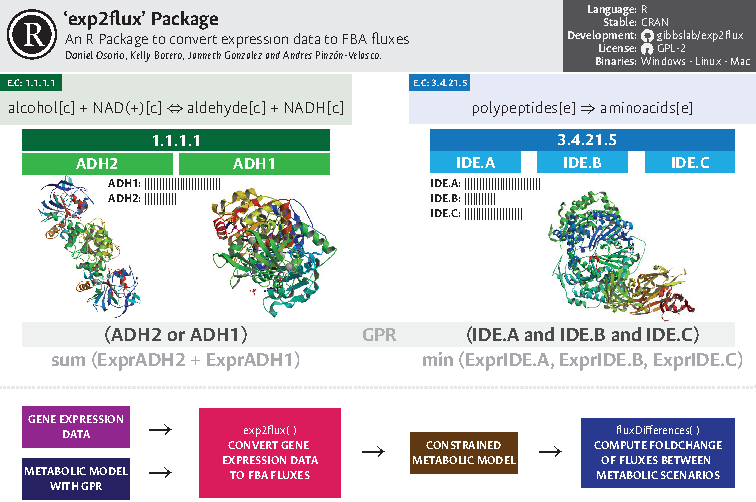
\includegraphics[width=\textwidth]{exp2flux}
\end{center}
\end{frame}
\section{Conclusion}
\begin{frame}

\end{frame}
\section{Events}
\begin{frame}{Advances of this work were presented as:}
\begin{center}

\includegraphics[width=\textwidth]{Events}
\end{center}
\hrulefill \ at: \hrulefill
\begin{multicols}{3}
\begin{center}
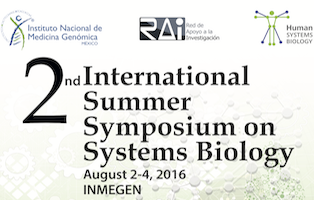
\includegraphics[width=0.3\textwidth]{IS3B}\\
CDMX, México\\
\textbf{Short Talk}
\end{center}
\begin{center}

\includegraphics[width=0.3\textwidth]{ICSB}\\
Barcelona, España\\
\textbf{Poster}
\end{center}
\begin{center}

\includegraphics[width=0.3\textwidth]{ICGEB}\\
Bogotá, Colombia\\
\textbf{Short Talk}
\end{center}
\end{multicols}
\end{frame}
\section{Questions}
\begin{frame}{This study is under development at the:}
\begin{multicols}{2}

\includegraphics[height=0.7cm]{logoIG}
\begin{flushright}

\includegraphics[height=0.7cm]{logoGIBBS}
\end{flushright}
\end{multicols}
\begin{center}
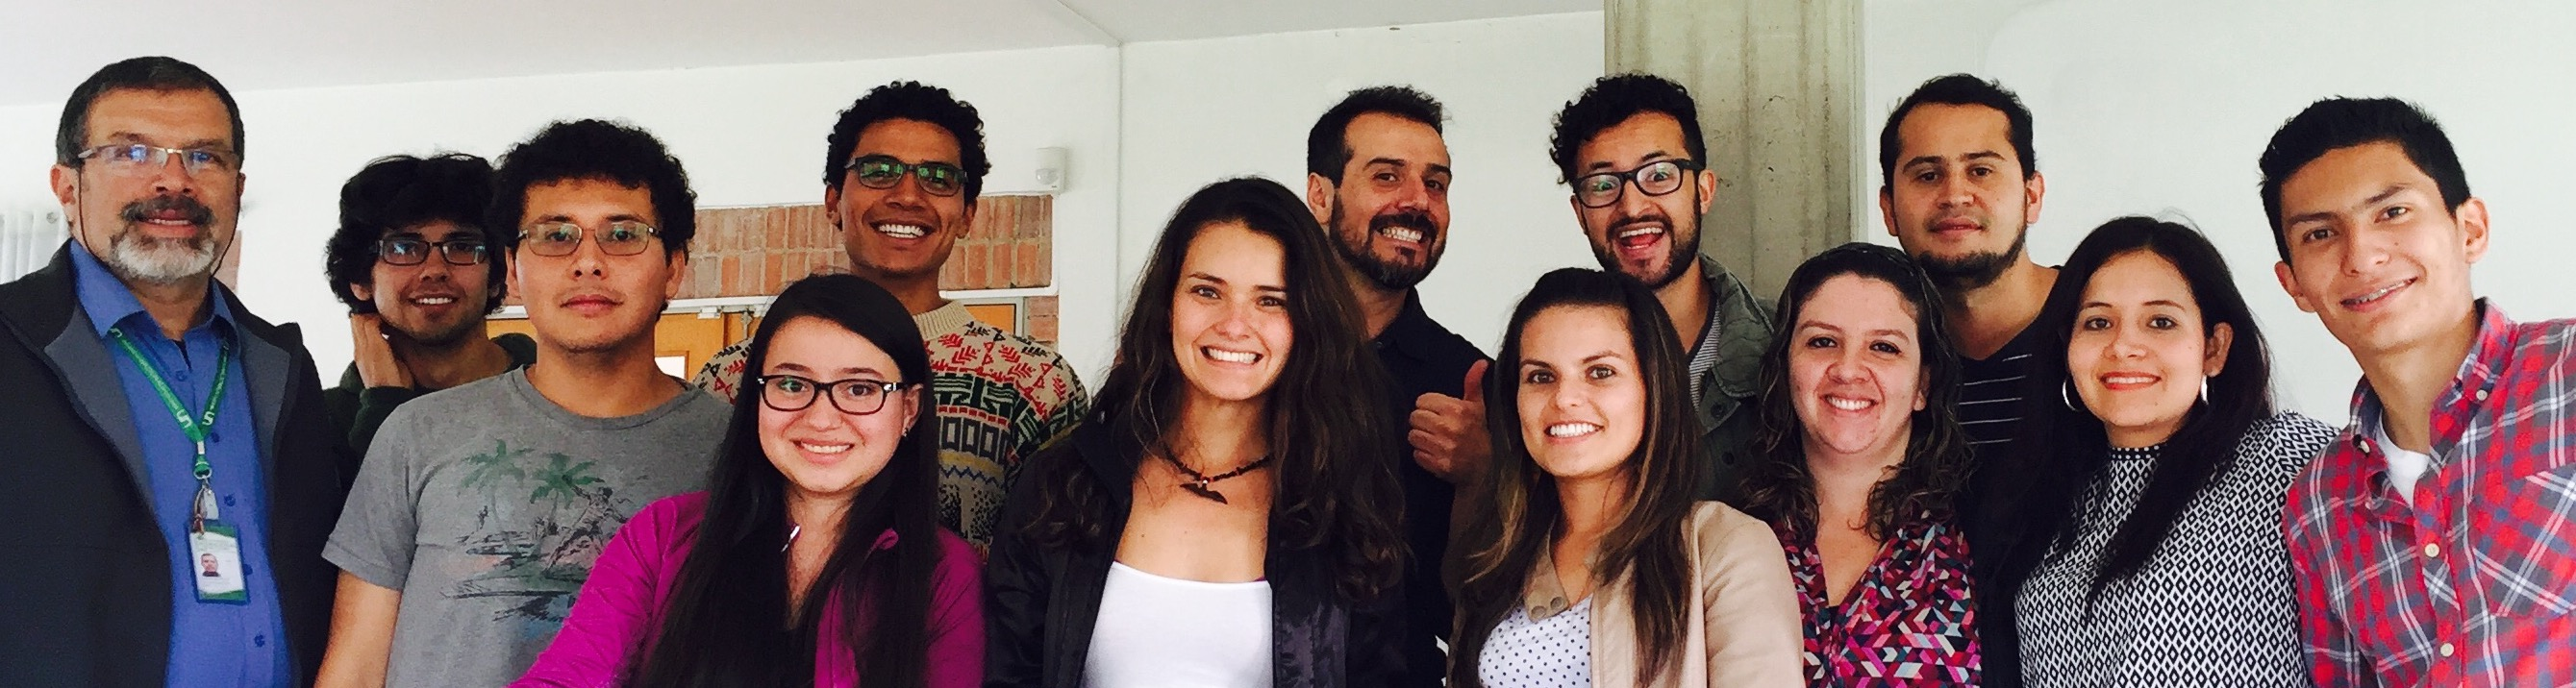
\includegraphics[width=\textwidth]{GIBBS}\\
\textbf{Bioinformatics and Computational Systems Biology Lab}\\
Institute for Genetics - Universidad Nacional de Colombia
\end{center}
\begin{center}
\textbf{CONTACT:}
\begin{multicols}{2}
\begin{center}
\textbf{Daniel Osorio}\\
dcosorioh@unal.edu.co\\
\textbf{Andrés Pinzón PhD}\\
ampinzonv@unal.edu.co
\end{center}
\end{multicols}
\end{center}
\end{frame}
\end{document}